\section{Results and Discussion}
\label{chapter:signalgp:sec:results-and-discussion}

\subsection{Changing Environment Problem}


\begin{figure*}[!ht]
  \centering 
  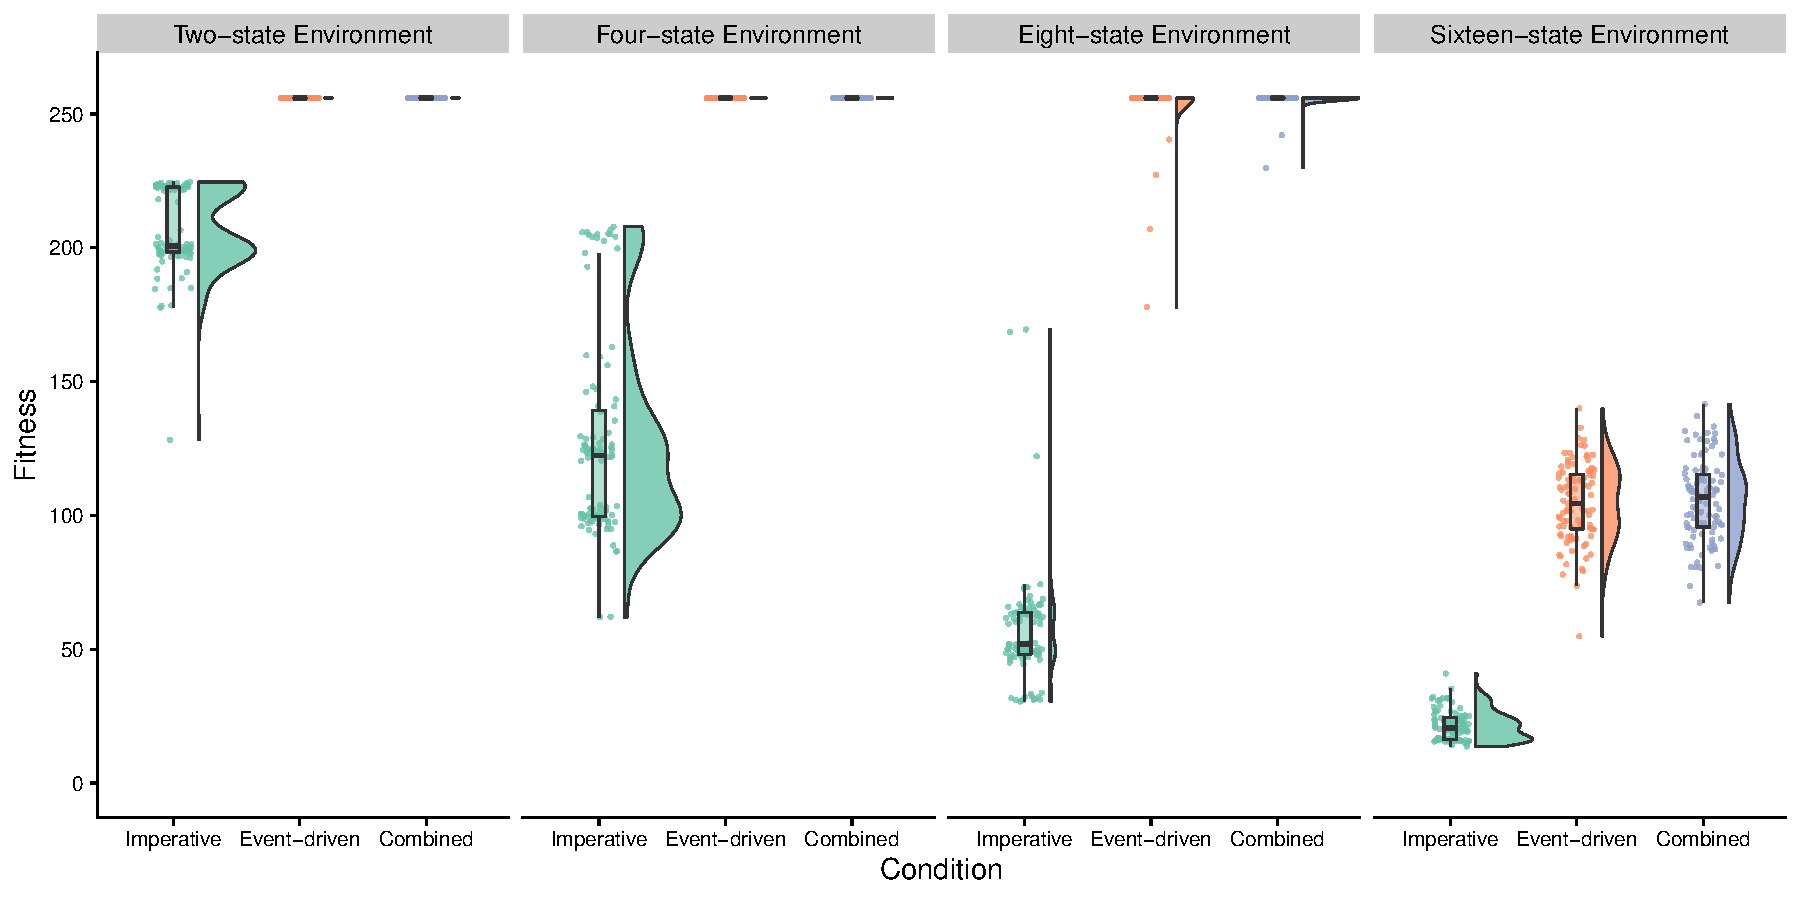
\includegraphics[width=\textwidth]{chapters/04-evolving-event-driven-programs-with-signalgp/media/chg-env-fitness.pdf}
  \caption{\small 
  Changing environment problem results across all environments: two-state environment, four-state environment, eight-state environment, and sixteen-state environment. 
  The raincloud plots \citep{allen_raincloud_2019} indicate the fitnesses (each an average over 100 trials) of best performing programs from each replicate.
  }
  \label{chapter:signalgp:fig:chg-env-fitness}
\end{figure*}


\subsubsection{Event-driven strategies outperform imperative strategies}

Figure \ref{chapter:signalgp:fig:chg-env-fitness} shows results for all environment sizes ($K$ = 2, 4, 8, and 16). 
Programs evolved in treatments with fully event-driven SignalGP significantly outperformed those evolved in the imperative treatment across all environments ($p<10^{-4}$ for all conditions). 
% : two-state (combined and event-driven, $p<10^{-4}$), %(combined: $p<2$e-47; event-driven: $p<2$e-47), 
% four-state (combined and event-driven, $p<10^{-4}$), %(combined: $p<2$e-47; event-driven: $p<2$e-47), 
% eight-state (combined and event-driven, $p<10^{-4}$), %(combined: $p<2$e-46; event-driven: $p<3$e-45), 
% and sixteen-state (combined and event-driven, $p<10^{-4}$), %(combined: $p<2$e-34; event-driven: $p<3$e-33). 
Across all environments, there was no significant difference in final program performance between the event-driven and combined treatment. 
See supplementary material for full details on statistical test results \citep{signalgp_supplement_2018}. 

Further, only treatments with fully event-driven SignalGP produced programs capable of achieving a perfect fitness of 256. 
This result is not surprising, as \textit{only} programs that employ an entirely event-driven strategy can achieve a perfect score in multi-state environments. 
This is because imperative strategies must continuously poll the environment for changes, which decreases the efficiency of their response to an environmental change.
This strategy becomes increasingly cumbersome and inefficient as the complexity of the environment increases. 
In contrast, event-driven responses are triggered automatically \textit{via} the SignalGP virtual hardware, facilitating immediate reactions to environmental changes.
This allows event-driven strategies to more effectively scale with environment size than imperative strategies. 

\subsubsection{Evolution favors event-driven strategies}

In the combined treatment, evolution had access to both the event-driven (signal-based) strategy and the imperative (sensor-polling) strategy. 
As shown in Figure \ref{chapter:signalgp:fig:chg-env-fitness}, performance in the combined treatment did not significantly differ from the event-driven treatment, but significantly exceeded performance in the imperative treatment. 
However, this result alone does not reveal what strategies were favored in the combined treatment. 

%What strategy did evolution favor in the combined treatment? 
To tease this apart, we re-evaluated programs evolved under the combined treatment in two distinct conditions:
one in which we deactivated sensors and one in which we deactivated external events. 
In the deactivated sensors condition, \code{SenseEnvState} instructions behaved as no-operations, which eliminated the viability of a sensor-based polling strategy.
Likewise, the deactivated events re-evaluation condition eliminated the viability of event-driven strategies.  
Any loss of functionality by programs in these new environments will tease apart the strategies that those programs must have employed.

\begin{figure}[h]
  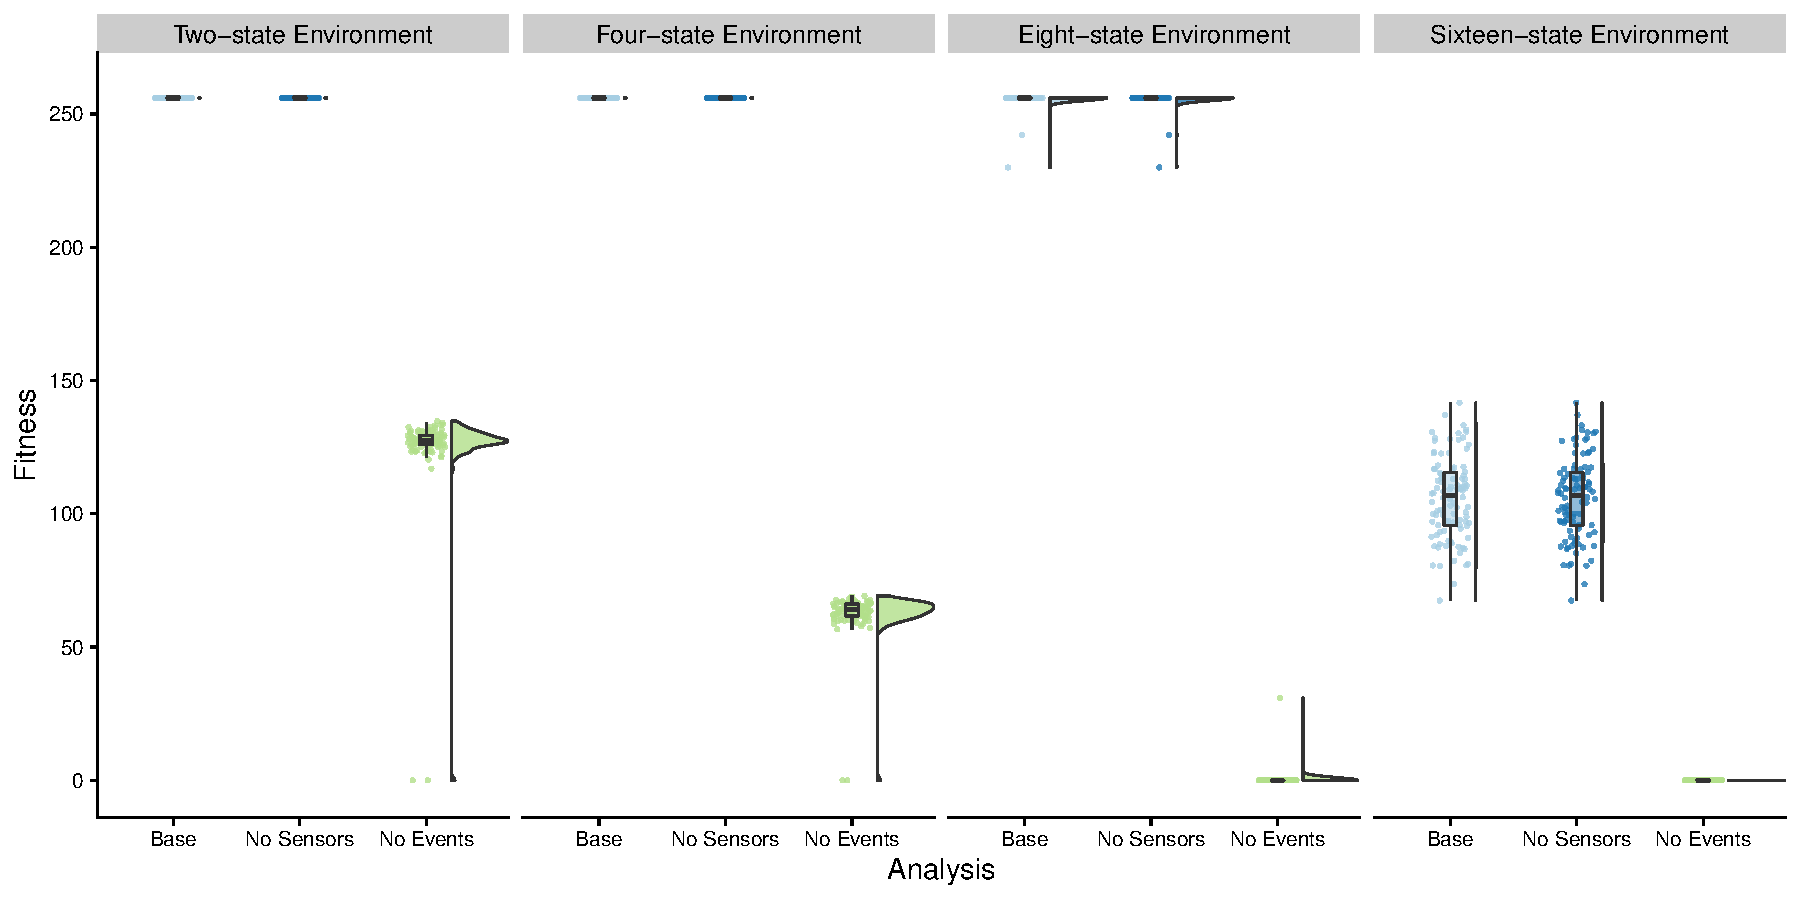
\includegraphics[width=\columnwidth]
  {chapters/04-evolving-event-driven-programs-with-signalgp/media/chg-env-combined-strategy.pdf}
  \caption{\small 
  Re-evaluation results for combined condition in the changing environment problem across all environments:  two-state environment, four-state environment, eight-state environment, and sixteen-state environment. 
  The raincloud plots indicate the fitnesses (each an average over 100 trials) of best performing programs from each re-evaluation.
  }
  \label{chapter:signalgp:fig:combined-reeval}
\end{figure}

Figure \ref{chapter:signalgp:fig:combined-reeval} shows the results of our re-evaluations. 
Across all environment sizes, there was no significant difference between program performance in their original combined condition and the deactivated sensors conditions. 
In contrast, program performances were significantly worse in the deactivated events condition than in the combined condition (all conditions, $p<10^{-4}$).
% (two-state: $p<2$e-47; four-state: $p<2$e-47; eight-state: $p<7$e-49 ; sixteen-state: $p<4$e-35). 
These data indicate that programs evolved in the combined condition primarily rely on event-driven strategies for the changing environment problem. 

\subsection{Distributed Leader Election Problem}

\begin{figure}[h]
  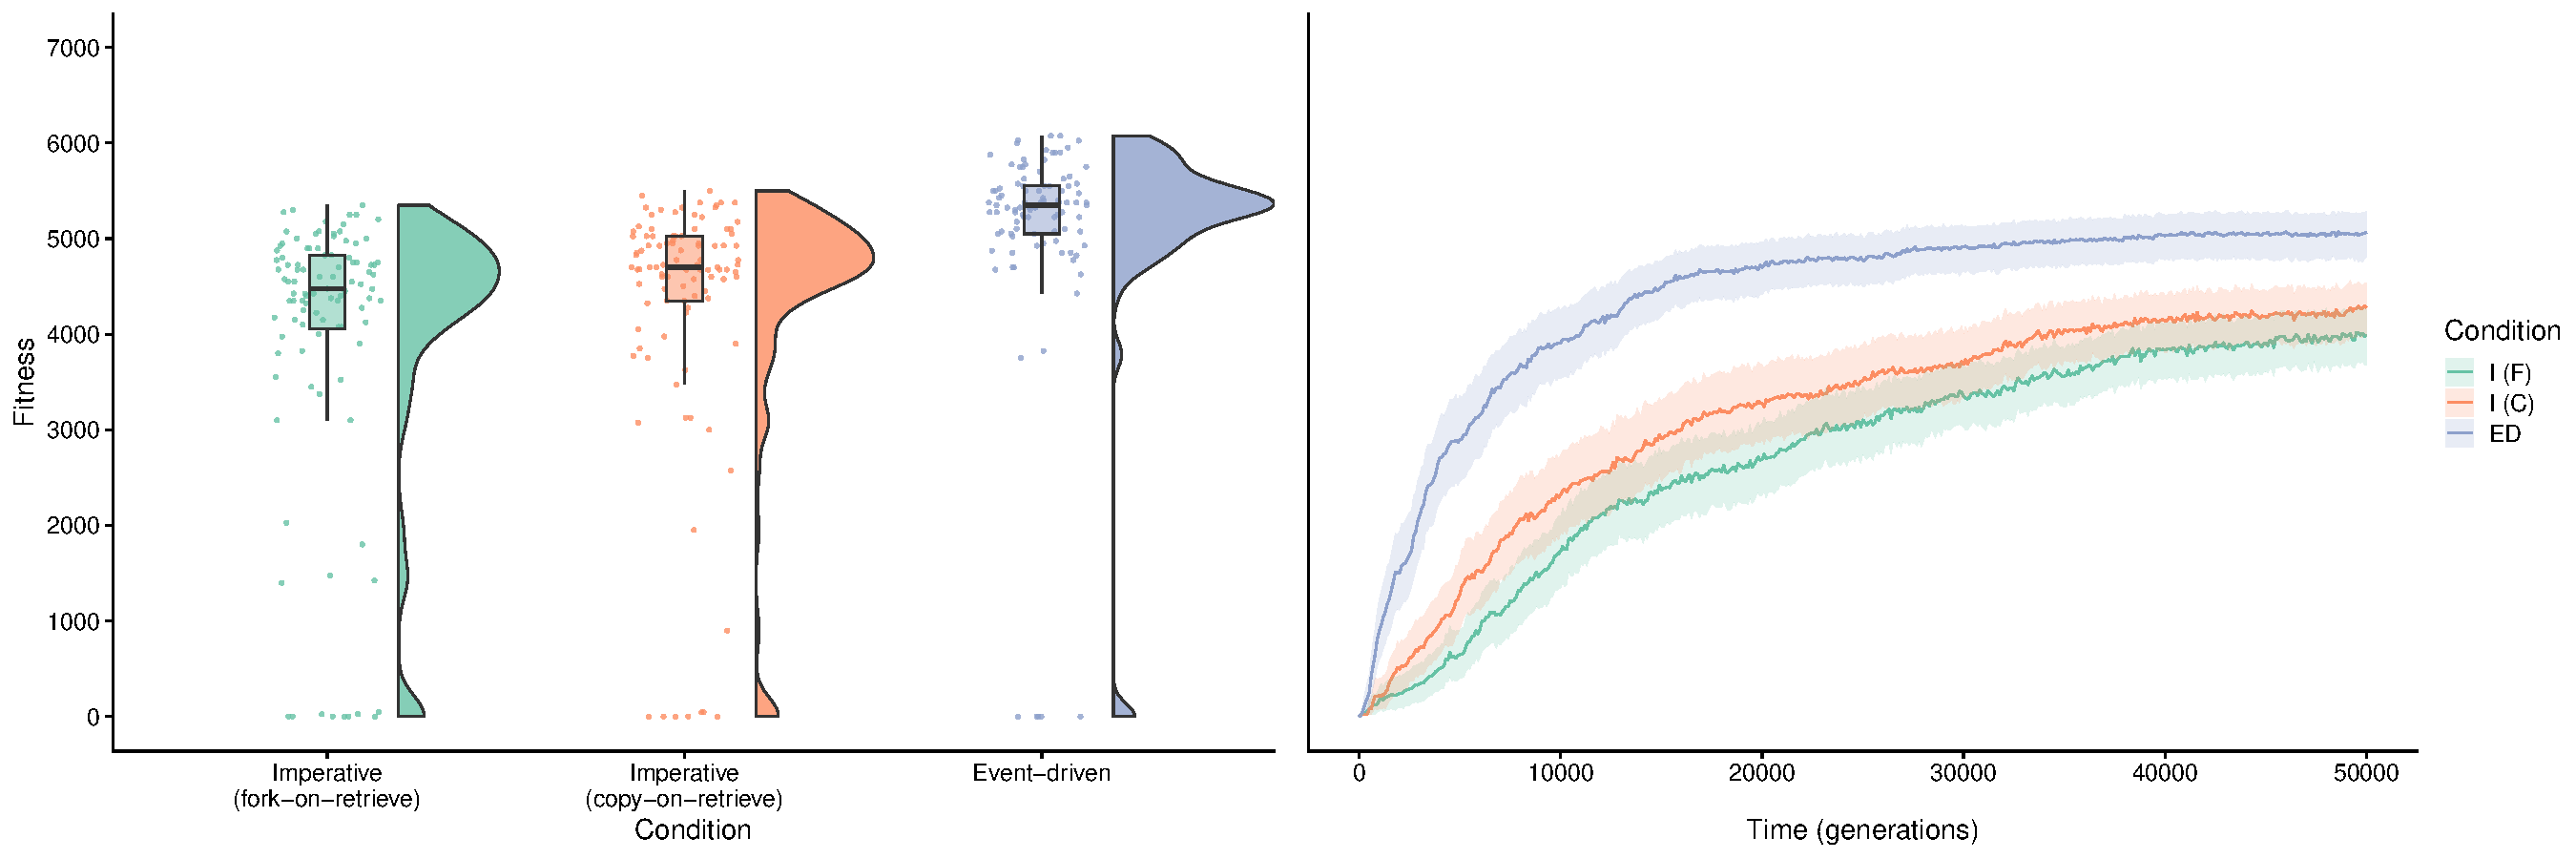
\includegraphics[width=\columnwidth]{chapters/04-evolving-event-driven-programs-with-signalgp/media/election-fitness.pdf}
  \caption{\small 
  Distributed leader election problem results. 
  The raincloud plots indicate the fitnesses of best performing distributed systems from each replicate. 
  The time series gives average fitness over time during evolution. 
  The colors in the time series correspond to the colors in the raincloud plots. 
  The shading on fitness trajectories in the time series indicates a bootstrapped 95\% confidence interval.
  }
  \label{chapter:signalgp:fig:election-fitness}
\end{figure}

% \vspace{2mm}
% \noindent\textbf{Event-driven networks outperform imperative networks.}\\
\subsubsection{Event-driven networks outperform imperative networks}

Figure \ref{chapter:signalgp:fig:election-fitness} shows the results for the distributed leader election problem.
Distributed systems evolved in the event-driven treatment significantly outperformed those evolved in both imperative treatments 
(fork-on-retrieval and copy-on-retrieval, $p<10^{-4}$). 
% (fork-on-retrieval: $p<2$e-21; copy-on-retrieval: $p<2$e-13). 
See supplementary material for full details on statistical test results \citep{signalgp_supplement_2018}. 

All three conditions produced distributed systems capable of achieving election consensus. 
The difference in performances across treatments primarily reflect how quickly consensus is able to be reached within a distributed system. 
The event-driven programming paradigm is able to more efficiently encode communication between agents, as it does not require programs to continuously poll for new messages from other agents. 
Thus, the event-driven paradigm allows signals to propagate more quickly through a distributed system than the imperative paradigm. 
The time series shown in Figure \ref{chapter:signalgp:fig:election-fitness} hints that the event-driven SignalGP representation evolves more rapidly for the distributed leader election problem than the imperative variants; however, deeper analyses are required for confirmation. 

